%Written by: Aaron Stillmaker
%September 11, 2018
%ECE 186A - Senior Design
%
%This is a template you can use for your Project Descriptions, though you will need to change a good portion of it for your own needs.

\documentclass{IEEEtran}					%Everything is default, which is journal, 10pt font, and final draft
\usepackage{dtk-logos}						%This let me do the cool BibTeX logo, you shouldn't need this line. Add additional packages here:
\usepackage{graphics}
\usepackage{caption} 
\usepackage{natbib}
\captionsetup[table]{skip=10pt}
\title{\vspace{2in}The Smart Eraser}	%the \vspace is moving the title down from the top of the page
\author{ECE 186A - Senior Design I \\ 			%I am jamming all of the stuff I want on the title page into the Author spot, I know, 
	%this isn't elegant.
	Fall 2018 - Dr. Stillmaker \\ 				%Note the \\ line returns to make sure to put each one on a new line
	\vspace{12pt} 								%I put in some space to get the due date listed a little lower
	\textbf{Date:} Friday, September 28, 2018  \\ 
	\vspace{2in}								%You may need to mess with this space, this space is above the signature lines.
	\vspace{6pt}
	\textbf{Project Manager:} Heather Libecki			%Uncomment this section and fill in your team names and your technical advisor's name.
	\vspace{12pt}
	\underline{\hspace{3in}}\\					%You are welcome to have more than one technical advisor if you wish..
	\textbf{Team Member:} Chris Quesada
	\vspace{12pt}
	\underline{\hspace{3in}}\\
	\textbf{Team Member:} Juan Colin
	\vspace{12pt}
	\underline{\hspace{3in}}\\
	\textbf{Technical Advisor:} Dr. Kulhandjian
	\underline{\hspace{3in}} \\
	\vspace{12in}}								%You will need to mess with this space, this space is after the signature lines.  The idea
%is to make the title page by itself.  I know, this isn't elegant either, but IEEE %formatting doesn't make title pages

\begin{document}
	\thispagestyle{empty}						%This removes the page number from the title page.
	
	\maketitle									%This generates the title from the information given above.
	
	
	\section{Introduction}
	\setlength{\parindent}{5ex}
	Our project, the Smart Eraser, is an automatic whiteboard eraser. The main deliverable of this project will be an eraser which can move left-to-right on a track, and up-and-down on a bar attached to the track. This eraser will be able to automatically detect on a whiteboard where there are markings through the use of a camera and image-detection programming. The camera will send the coordinates of the markings to the eraser, which will then find the quickest route to erase the markings, before returning to its stand-by position. The eraser will also be able to detect the presence of a person, resulting in the immediate termination of whatever process it was carrying out.\par
	\setlength{\parindent}{5ex}	
	Heather Libecki is responsible for being the project manager, the wireless communication between the camera and the imbedded system, and she will also be contributing to the completion of the image-processing program which will detect where the markings on the board are. Chris Quesada is responsible for developing the microcontroller code, particularly the physical movement protocols of the system, using the coordinates specified by the camera, and he will also be contributing to the completion of the image-processing program which will detect if a person is in front of the board. Juan Colin is responsible for the creation and execution of the physical, mechanical system that the eraser will be attached to, including the wiring of the system itself, and he will also be contributing to the research and implementation of the power system. All three of the team members will assist each other with the initial research, then break off into their own specialties as the project completion progresses.
	
	\section{Background}
	The main goal of this project is to create a fully-functional automatic eraser that detects where it needs to erase as well as if there is a person in front of the board. The following objectives will need to be accomplished in order to obtain this goal: design a track system for the eraser, design a power system for the track, design a control panel/interface, create a compact unit that can easily be moved on the track, create an image-processing program in Matlab, create the path/coordinate system for the eraser to follow, communicate the created path to the microcontroller, and detect if a person is standing in front of the board.
	The following list contains the strengths and weaknesses that were found for each member of the group.\\\\
	Heather Libecki
	\begin{itemize}
		\item Strengths: programming (assembly, Matlab), mathematics, debugging, circuit implementation, problem solving, technical writing, public speaking
	 	\item Weaknesses: programming (verilog, Python), circuitry design, coding algorithms, power systems, Github
 	\end{itemize}
 	Chris Quesada
	\begin{itemize}
		\item Strengths: programming (assembly, verilog, Matlab) embedded systems, algorithms, Github, brainstorming
		\item Weaknesses: programming (Python), circuitry design, mathematics, public speaking
	\end{itemize}
	Juan Colin
	\begin{itemize}
		\item Strengths: electrical systems, circuitry design, problem solving, power systems, public speaking/relations
		\item Weaknesses: programming (assembly, verilog, Matlab, Python), Github, technical writing and spelling \\
	\end{itemize} 
	\par
	\setlength{\parindent}{5ex} 
	The background information that will need to be researched in order to implement this project is: image-processing programs, translating data from image-processing into coordinates, wireless communication between separate devices, Simulink in Matlab, Github repositories, Python usage, connecting physical devices for the track of the eraser, language and usage of Raspberry Pi, and other research as necessary. The specific courses that this group has taken that will be used in the implementation of this project are: 
	\subsection{Embedded Systems (ECE 178)}
	\begin{itemize}
		 \item System creation and customization in QSYS, developement of algortithms, setting up and using interrupts, interfacing with periphereals on the board.
	\end{itemize}
	\subsection{Introduction to Electrical and Computer Engineering Tools (ECE 72)} 
	\begin{itemize}
		\item Navigating and using MATLAB/Simulink.
	\end{itemize}
	\subsection{Computer Networks (ECE 146)} 
	\begin{itemize}
		\item Determining how to use blue tooth to setup connections between micro controller, camera, and possibly control panel. The communication between all parts of the project will be one of main obstacles of the project.
	\end{itemize}
	\subsection{Principles of Electrical Circuits (ECE 90)}
	\begin{itemize}
		\item Developing the power scheme and parameters for the stepper motors and track system. Also, if time permits, developing the power system for the control panel.
	\end{itemize}
	\subsection{Microprocessor Architecture and Programming (ECE 118)}
	\begin{itemize}
		\item Using the recursion technique and algorithms developed when the shortest-tree path was covered, determining how much memory and how data is stored into memory, and working with an ARM processor.
	\end{itemize}
	\subsection{Digital Logic Design (ECE 85)}
	\begin{itemize}
		\item If time permits, developing a PCB for the control  panel based on designs from the state machine development (next section), determining various connections between stepper motors, micro controller, track system and power source.
	\end{itemize}
	\subsection{Switching Theory and Logical Design (ECE 106)}.
	\begin{itemize}
		\item If time permits ,development of a state machine that will act as a control panel, and developing flow charts and diagrams of the overall system.
	\end{itemize}
	\section{Project Description}
	\subsection{Design track system}
	The figure shown below is a rough layout of what the final deliverable will look like. The arrow labeled {\lq}1{\rq} is the eraser connected to the pole that will move it up and down, the arrows labeled {\lq}2{\rq} is the track system that will be mounted above and below the whiteboard, and will allow the eraser to move left and right, and the arrow labeled {\lq}3{\rq} shows the writing on the board that will be erased.
	\begin{figure}[h!]
	\resizebox{8cm}{!}
	{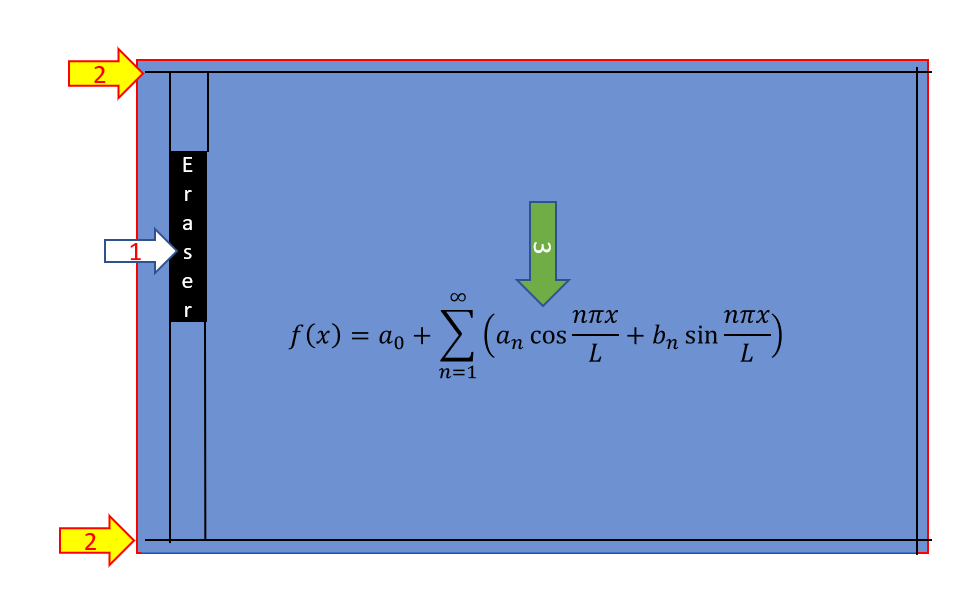
\includegraphics{Diargram one.png}}
	\caption{How the smart eraser will be attached to the white board.}
	\label{fig:look}
	\end{figure}
	
	\subsection{Design a power system}
	The eraser needs to have a power system that will allow it to stay active whenever it is needed, and the camera will as well. The eraser will more than likely be connected to a power source (like a wall outlet) because the power consumption of this product will be too much for a standard battery to keep charged for an extended period of time. This power system would need to have a range of motion, meaning there would need to be cords long enough to connect to the eraser without limiting its range of motion, so it can move freely without the risk of becoming unplugged. 
	\subsection{Configure MATLAB to Communicate with FPGA}
	Using Mathworks information and references, an FPGA device will be configured so it will work with Matlab code. The specific FPGA board that will be used is the DE2-115 development board. First, we would set up the synthesis tool path within Matlab, which is also known as the HDL coder. Upon completion, this will allow a connection to be established between the computer and the development board. After creating a new project, which involves a function and testbench file, the HDL workflow advisor will then be used to correctly communicate with the board and run Matlab code on it as well. Integration of the board with Matlab will be advantageous because of its image processing toolbox.
	
	\subsection{Configure bluetooth connection via MATLAB}
	In order to receive images from the camera for processing, a bluetooth connection will need to be established so the information can be transmitted wirelessly. This connection will be established via a USB bluetooth dongle which will be plugged into the FPGA, and Mathworks provides additional information on how to establish this connection, which is another reason why Matlab will need to be integrated with the FPGA.
	\subsection{Process an image in Matlab}
	The primary reason for using Matlab in this project is to take advantage of the image processing capabilities it has to offer through its image processing toolbox. There will be an external camera pointing at the board which will capture an image, transmit that image{\rq}s data via a wireless bluetooth connection to the DE2-115 microcontroller, and there the image will be processed in a Matlab code. This will allow the eraser to move to where the markings are on the board in a ``smart'' way. The most convenient mode of image processing for the purposes of this project is to convert the image to a grayscale version of itself, which will allow for an easy detection of where any outlying markings are located. Their location will be converted into coordinates for the eraser to follow. The main obstacle of this objective is creating the algorithm which takes the marking{\rq}s locations and converts them to a coordinate system that the eraser will be able to utilize. Another obstacle is figuring out a way to make sure the eraser takes the shortest path possible when erasing the marks, in order to keep the system efficient.
	
	\subsection{Create a path to follow based on the image processing done in Matlab}
	In the previous objective, it was stated that the eraser should follow the shortest path possible when erasing the markings, which means it will be taking a ``smart-path''. This means that the program will need to find the shortest, quickest path possible while reaching all the coordinates that need to be erased. This can be accomplished by finding the shortest path between a source node (or coordinate) to all other nodes in the graph; this is also known as the shortest-path tree. There are many algorithms that can accomplish this, and information from the ECE catalog{\rq}s microprocessor course will also aid in the completion of this objective. It was decided that this ``smart-path'' should be created because it provides more of a challenge to the project. Otherwise, it would be relatively simple to create a random path for the eraser to follow, or even just programming it to move back and forth to erase the entire board every time it is activated.
	
	\subsection{Communicate path via FPGA to track system}
	There will be two stepper motors that work in conjunction to drive the track system, and they need to be able to communicate with the FPGA. This will be done via the GPIO pins attached to the board, which are also known as the expansion header. Using the Reference Manual provided from Altera, this system component will be configured to send the smart-path data to the stepper motors via an H-Bridge. The H-bridge is necessary to drive the motors forwards or backwards. This is done by turning a specific combination of the 4 switches on or off, which will allow the polarity of the voltage being applied to the load to change. 
	
	\subsection{Drive stepper motors to move track system along path}
	Another one of the larger obstacles that needs to be overcome is translating the smart-path to a usable coordinate system which will allow the stepper motors to move the eraser to the correct position on the board. When completed, it should move the way a vinyl plotter does, which works by having a track that can move left and right, and a roller that can move it up and down, to cover all directions of a 2D grid. The two stepper motors will need to be able to accomplish this for the Smart Eraser. The algorithm that converts the processed image into coordinates will need to be expressed in terms of rotation patterns in order to move the eraser correctly to the desired location.
	
	\subsection{Implement movement detection}
	A potential safety issue concerns the movement of the eraser while someone is by, or using, the whiteboard. In order to prevent any potential bodily collisions with the device while it is in motion, there will need to be a movement detection system put into place. This detection system will make the eraser stop moving wherever it is whenever a person is standing in front of the whiteboard. The best way to accomplish this is to set up an ISR (interrupt service routine) which will be communicated with the camera. In addition, the camera will need to take an image and send it to the FPGA every second or so to detect a change in the image, so a subroutine comprised of this logic will also need to be created. If movement is detected, an interrupt will be issued in order to halt the eraser{\rq}s motion. The eraser{\rq}s original task will resume when there is no more movement being detected, or when there is a physical override detected from a programmed pushbutton.
	
	\subsection{Estimated Costs}
	\begin{table} [h!]	
		\centering
		\resizebox{8cm}{!}{
		\begin{tabular}{|c|c|}
			\hline
			\textbf{Component} & \textbf{Est. Price} \\
			\hline
			Standard Eraser & \$3 \\
			\hline
			Standard Whiteboard & \$50 \\
			\hline
			Stepper Motors & \$60 x2 \\ 
			\hline 		
			H-bridge & \$2 \\
			\hline
			HD camera & varies \\
			\hline
			Metal Tracks & varies \\
			\hline
			Pulleys & varies \\
			\hline
			various wires and connections & varies \\
			\hline
		\end{tabular} }
		\caption{Estimated costs of components for project}
		\label{table:1}
					
	\end{table}		
	The technical advisor for this project is Dr. Hovannes Kulhandjian, who specializes in digital signal processing, and wireless communications and networking.	He will contribute advice and information pertaining to the bluetooth connectivity of the camera to the image processing microcontroller. Dr. Kulhandjian was the original mind behind the idea of this project as well. Because of this, he will also be contributing more specifications and features to the project as its completion progresses. 			
	\bibliographystyle{IEEEtran}
	\bibliography{references}	
	1.https://www.mathworks.com/help/supportpkg/alterafpgaturnkeyboards/ug/program-standalone-fpga-with-fpga-turnkey-workflow-from-.html\\\\
	2.https://www.mathworks.com/help/instrument/bluetooth-communication.html
		
\end{document}
